% Options for packages loaded elsewhere
\PassOptionsToPackage{unicode}{hyperref}
\PassOptionsToPackage{hyphens}{url}
%
\documentclass[
  10pt,
  ignorenonframetext,
]{beamer}
\usepackage{pgfpages}
\setbeamertemplate{caption}[numbered]
\setbeamertemplate{caption label separator}{: }
\setbeamercolor{caption name}{fg=normal text.fg}
\beamertemplatenavigationsymbolsempty
% Prevent slide breaks in the middle of a paragraph
\widowpenalties 1 10000
\raggedbottom
\setbeamertemplate{part page}{
  \centering
  \begin{beamercolorbox}[sep=16pt,center]{part title}
    \usebeamerfont{part title}\insertpart\par
  \end{beamercolorbox}
}
\setbeamertemplate{section page}{
  \centering
  \begin{beamercolorbox}[sep=12pt,center]{part title}
    \usebeamerfont{section title}\insertsection\par
  \end{beamercolorbox}
}
\setbeamertemplate{subsection page}{
  \centering
  \begin{beamercolorbox}[sep=8pt,center]{part title}
    \usebeamerfont{subsection title}\insertsubsection\par
  \end{beamercolorbox}
}
\AtBeginPart{
  \frame{\partpage}
}
\AtBeginSection{
  \ifbibliography
  \else
    \frame{\sectionpage}
  \fi
}
\AtBeginSubsection{
  \frame{\subsectionpage}
}
\usepackage{lmodern}
\usepackage{amssymb,amsmath}
\usepackage{ifxetex,ifluatex}
\ifnum 0\ifxetex 1\fi\ifluatex 1\fi=0 % if pdftex
  \usepackage[T1]{fontenc}
  \usepackage[utf8]{inputenc}
  \usepackage{textcomp} % provide euro and other symbols
\else % if luatex or xetex
  \usepackage{unicode-math}
  \defaultfontfeatures{Scale=MatchLowercase}
  \defaultfontfeatures[\rmfamily]{Ligatures=TeX,Scale=1}
\fi
\usetheme[]{Berlin}
% Use upquote if available, for straight quotes in verbatim environments
\IfFileExists{upquote.sty}{\usepackage{upquote}}{}
\IfFileExists{microtype.sty}{% use microtype if available
  \usepackage[]{microtype}
  \UseMicrotypeSet[protrusion]{basicmath} % disable protrusion for tt fonts
}{}
\makeatletter
\@ifundefined{KOMAClassName}{% if non-KOMA class
  \IfFileExists{parskip.sty}{%
    \usepackage{parskip}
  }{% else
    \setlength{\parindent}{0pt}
    \setlength{\parskip}{6pt plus 2pt minus 1pt}}
}{% if KOMA class
  \KOMAoptions{parskip=half}}
\makeatother
\usepackage{xcolor}
\IfFileExists{xurl.sty}{\usepackage{xurl}}{} % add URL line breaks if available
\IfFileExists{bookmark.sty}{\usepackage{bookmark}}{\usepackage{hyperref}}
\hypersetup{
  pdftitle={Do Gasoline Expenditure Shocks Have Different Effects in Recessions \& Expansions?},
  pdfauthor={Naafey Sardar\^{}1; Dr.~Lance Bachmeier\^{}2},
  hidelinks,
  pdfcreator={LaTeX via pandoc}}
\urlstyle{same} % disable monospaced font for URLs
\newif\ifbibliography
\usepackage{longtable,booktabs}
\usepackage{caption}
% Make caption package work with longtable
\makeatletter
\def\fnum@table{\tablename~\thetable}
\makeatother
\usepackage{graphicx,grffile}
\makeatletter
\def\maxwidth{\ifdim\Gin@nat@width>\linewidth\linewidth\else\Gin@nat@width\fi}
\def\maxheight{\ifdim\Gin@nat@height>\textheight\textheight\else\Gin@nat@height\fi}
\makeatother
% Scale images if necessary, so that they will not overflow the page
% margins by default, and it is still possible to overwrite the defaults
% using explicit options in \includegraphics[width, height, ...]{}
\setkeys{Gin}{width=\maxwidth,height=\maxheight,keepaspectratio}
% Set default figure placement to htbp
\makeatletter
\def\fps@figure{htbp}
\makeatother
\setlength{\emergencystretch}{3em} % prevent overfull lines
\providecommand{\tightlist}{%
  \setlength{\itemsep}{0pt}\setlength{\parskip}{0pt}}
\setcounter{secnumdepth}{-\maxdimen} % remove section numbering
\setbeamertemplate{page number in head/foot}[totalframenumber]

\title{Do Gasoline Expenditure Shocks Have Different Effects in Recessions \&
Expansions?}
\author{Naafey Sardar\(^1\) \and Dr.~Lance Bachmeier\(^2\)}
\date{}
\institute{\(^1\)Ph.D.~Candidate, Department of Economics, Kansas State University \and \(^2\)Associate Professor, Department of Economics, Kansas State
University}

\begin{document}
\frame{\titlepage}

\begin{frame}{Objective}
\protect\hypertarget{objective}{}

\begin{itemize}
\item
  What happens to non-gasoline consumption when there is a shock to
  gasoline expenditures?
\item
  Does the response of non-gasoline consumption to gasoline expenditures
  depend on the state of the business cycle?
\item
  Why is the response of non-gasoline consumption to gasoline
  expenditures different between recessions and expansions?
\end{itemize}

\end{frame}

\begin{frame}{What To Take Away}
\protect\hypertarget{what-to-take-away}{}

Using a structural VAR model for U.S. data covering the period
1973-2018, this paper shows that

\begin{itemize}
\item
  An increase in gasoline expenditures reduces aggregate consumption.
\item
  The response to a gasoline expenditure shock is much stronger in a
  recession than in an expansion.
\item
  The difference in response over the business cycle is due to the
  differences in household savings behaviour in recessions versus
  expansions.
\item
  Our results are consistent with the literature showing large effects
  of fiscal policy in recessions.
\end{itemize}

\end{frame}

\begin{frame}{Contributions}
\protect\hypertarget{contributions}{}

\begin{itemize}
\item
  This is the first paper to suggest that the effect of a gasoline
  expenditure shock depends on the state of the economy.
\item
  We present a novel forecasting model that accounts for this kind of
  asymmetry.
\item
  This model would allow the Federal Reserve to precisely estimate the
  effect of a gasoline expenditure shock on consumption (or other macro
  variable) in recessions and expansions.
\end{itemize}

\end{frame}

\begin{frame}{Relationship between U.S. Consumption and Gasoline
Expenditures (1973-2018)}
\protect\hypertarget{relationship-between-u.s.-consumption-and-gasoline-expenditures-1973-2018}{}

\begin{figure}
\centering
\includegraphics[width=0.8\textwidth,height=\textheight]{Shares of Consumption.png}
\caption{Gasoline and Non-Gasoline Shares of Consumption}
\end{figure}

\end{frame}

\begin{frame}{Relationship between U.S. Consumption and Gasoline
Expenditures (1973-2018)}
\protect\hypertarget{relationship-between-u.s.-consumption-and-gasoline-expenditures-1973-2018-1}{}

\begin{itemize}
\tightlist
\item
  Gasoline share of consumption peaked in the early 1980's.
\item
  Low and stable global oil prices contributed to low shares during the
  1990's.
\item
  The more recent increase came in the early 2000's when oil prices
  increased due to high global oil demand.
\end{itemize}

\end{frame}

\begin{frame}{Relationship between U.S. Consumption and Gasoline
Expenditures (1973-2018)}
\protect\hypertarget{relationship-between-u.s.-consumption-and-gasoline-expenditures-1973-2018-2}{}

\begin{itemize}
\item
  A key question in macroeconomics is how aggregate consumption responds
  to a shock to gasoline expenditures?
\item
  If gasoline consumption is inelastic in the short-run, a positive
  shock to gasoline price will lead to higher gasoline expenditures,
  reducing spending on non-gasoline goods and services.

  \begin{itemize}
  \tightlist
  \item
    Hamilton (2009): Less discretionary income available as gasoline
    expenditures rise.\\
  \item
    Hamilton (1988): As gasoline expenditures increase, demand for
    energy-consuming goods falls.
  \item
    Farrell and Greig (2015): The MPC for non-energy goods is 0.8 for
    every dollar saved on gasoline.
  \item
    Gicheva et al.~(2008): Higher gasoline expenditures affects
    consumers spending on food.
  \end{itemize}
\end{itemize}

\end{frame}

\begin{frame}{U.S. Net Imports of Crude Oil (1973-2018)}
\protect\hypertarget{u.s.-net-imports-of-crude-oil-1973-2018}{}

\begin{figure}
\centering
\includegraphics[width=0.7\textwidth,height=\textheight]{Net Imports.png}
\caption{U.S. Net Imports of Crude Oil and Petroleum Products}
\end{figure}

\begin{itemize}
\item
  Increase in gasoline expenditures have caused a transfer of U.S.
  income to foreign oil producers.
\item
  Higher gasoline expenditures have the same effect as a tax on the U.S.
  economy and should be expected to reduce aggregate consumption.
\end{itemize}

\end{frame}

\begin{frame}{U.S. Net Imports of Crude Oil}
\protect\hypertarget{u.s.-net-imports-of-crude-oil}{}

\begin{itemize}
\tightlist
\item
  Jannet Yellen (2011):
\end{itemize}

``A higher price of imported oil is the equivalent of a tax on
consumers. It is a transfer from US consumers to foreign oil producers.
The effect should be the same as a tax increase. This tends to have a
dampening effect on consumer spending.''

\begin{itemize}
\tightlist
\item
  S\&P Global Economists Beth Bovino and Satyam Panday (2018):
\end{itemize}

``This would be tantamount to a tax increase for American households.''

\end{frame}

\begin{frame}{Fiscal Policy Literature}
\protect\hypertarget{fiscal-policy-literature}{}

\begin{itemize}
\item
  The motivation for our analysis is the recent literature showing that
  the impact of fiscal policy depends on the state of the economy.
\item
  Tagkalakis (2008): Tax cuts are more effective in boosting private
  consumption in recessions.
\item
  Auerbach and Gorodnichenko (2012): Fiscal multipliers are larger in
  recessions than expansions.
\item
  Jorda and Taylor (2016): Fiscal austerity depresses the economy more
  in a slump as opposed to a boom.
\end{itemize}

\end{frame}

\begin{frame}{Motivation}
\protect\hypertarget{motivation}{}

\begin{itemize}
\item
  Due to the oil-importing nature of the U.S. economy, shocks to
  gasoline expenditures have the same effect as a change in taxes.
\item
  Fiscal policy has different effects in recessions and expansions.
\item
  It follows that the effect of a gasoline expenditure shock should
  depend on the state of the business cycle.
\end{itemize}

\end{frame}

\begin{frame}{Why Should We Care?}
\protect\hypertarget{why-should-we-care}{}

\begin{itemize}
\item
  A finding of economically meaningful asymmetry of this type requires a
  change to empirical and theoretical macroeconomic models that include
  energy prices.
\item
  Implications for consumption forecasting.
\item
  A failure to find evidence would cast doubt on the following:

  \begin{itemize}
  \tightlist
  \item
    Treatment of a gasoline expenditure shock as a change in taxes.
  \item
    Claims that the effect of fiscal policy depends on the state of the
    economy.
  \item
    Both claims.
  \end{itemize}
\end{itemize}

\end{frame}

\begin{frame}{Linear Model}
\protect\hypertarget{linear-model}{}

We begin the analysis by estimating a (linear) bivariate structural VAR
model,

\[z_{t}=\alpha+\sum_{i=1}^{p}\beta_{i}z_{t-i}+e_{t}\]

\begin{itemize}
\tightlist
\item
  \(z_{t}=(\Delta gas_{t}, \Delta c_t)^{\prime}\)
\item
  \(\Delta gas_{t}\) is the percentage change in gasoline expenditures
  in quarter t
\item
  \(\Delta c_{t}\) is a measure of consumption growth in quarter t
\item
  \(e_{t}=(e_{gas,t}, e_{c,t})'\) is a vector of reduced form residuals
\item
  p represents the lag-length, whereas \(\alpha\) and \(\beta_{i}\) are
  vectors of coefficients.
\end{itemize}

\end{frame}

\begin{frame}{Linear Model}
\protect\hypertarget{linear-model-1}{}

\begin{itemize}
\item
  Gasoline expenditures are defined as the real personal consumption
  expenditures on gasoline goods and services.
\item
  The four measures of consumption growth we use are:

  \begin{itemize}
  \tightlist
  \item
    RPCE
  \item
    RPCE: Durables
  \item
    RPCE: Nondurables
  \item
    RPCE: Services
  \end{itemize}
\item
  Estimation of the linear VAR model does not represent an original
  contribution.
\item
  It provides a benchmark for comparison with results of the nonlinear
  model.
\end{itemize}

\end{frame}

\begin{frame}{Data Transformation}
\protect\hypertarget{data-transformation}{}

\begin{itemize}
\item
  Data on consumption was downloaded from National Income and Product
  Accounts (NIPA) tables.
\item
  Nominal variables are deflated using the \emph{Price Index for PCE}
  and transformed into real variables.
\item
  We conduct stationarity tests like the Augmented DF, Phillips-Perron,
  and ERS modified DF test.
\item
  Results suggest that the real consumption variables are non-stationery
  in levels but stationery in percentage differences.
\end{itemize}

\end{frame}

\begin{frame}{Data Transformation}
\protect\hypertarget{data-transformation-1}{}

\begin{figure}
\centering
\includegraphics[width=0.7\textwidth,height=\textheight]{Unit Root - Levels.jpg}
\caption{All tests include an intercept and a linear trend. 5\% critical
values for the respective tests are: -3.42, -2.89, -3.42.}
\end{figure}

\end{frame}

\begin{frame}{Data Transformation}
\protect\hypertarget{data-transformation-2}{}

\begin{figure}
\centering
\includegraphics[width=0.7\textwidth,height=\textheight]{Unit Root - Diff.jpg}
\caption{All tests include an intercept and a linear trend. 5\% critical
values for the respective tests are: -3.42, -2.89, -3.42.}
\end{figure}

\end{frame}

\begin{frame}{Identification of the Linear Model}
\protect\hypertarget{identification-of-the-linear-model}{}

\begin{itemize}
\item
  Our ordering of the variables implies a recursive system with gasoline
  expenditures ordered first.
\item
  Consumption responds contemporaneously to gasoline expenditures, and
  not vice versa.
\item
  The Cholesky decomposition of the variance-covariance matrix of
  reduced form residuals suggests that,
\end{itemize}

\[e_t=
\begin{pmatrix}
e_{gas,t}\\ 
e_{c,t}
\end{pmatrix}=
\begin{bmatrix}
1 & 0\\ 
a_{21} & 1 
\end{bmatrix}
\begin{pmatrix}
\varepsilon_{gas,t}\\ 
\varepsilon_{c,t}
\end{pmatrix}\]

\[e_{gas,t}=\varepsilon_{gas,t}\]
\[e_{c,t}=a_{21}\varepsilon_{gas,t}+\varepsilon_{c,t}\]

\end{frame}

\begin{frame}{Identification of the Linear Model}
\protect\hypertarget{identification-of-the-linear-model-1}{}

\begin{itemize}
\item
  Metric for judging the plausability of our assumption is to look at
  the contemporaneous correlations of the VAR residuals.
\item
  If gasoline expenditures are reacting immediately to macroeconomic
  shocks, it will cause a positive correlations between residuals.
\item
  On the other hand, if consumption expenditures are reacting to
  gasoline expenditures, the correlation will be negative.
\end{itemize}

\begin{longtable}[]{@{}lc@{}}
\toprule
Variables & Correlation (\(e_{gas,t}\), \(e_{c,t}\))\tabularnewline
\midrule
\endhead
RPCE & -0.35\tabularnewline
RPCE:Durables & -0.07\tabularnewline
RPCE:Nondurables & -0.26\tabularnewline
RPCE:Services & -0.45\tabularnewline
\bottomrule
\end{longtable}

\end{frame}

\begin{frame}{Interpretation of the Structural Shock}
\protect\hypertarget{interpretation-of-the-structural-shock}{}

What is the structural shock (\(\varepsilon_{gas,t}\)) capturing?

\begin{itemize}
\item
  Unanticipated changes in the price of gasoline.
\item
  Change in the preferences for larger or smaller vehicles.
\item
  Change in travel patterns.
\item
  Change in commuting behaviour due to fluctuations in house prices.
\end{itemize}

\end{frame}

\begin{frame}{Results: Linear Model}
\protect\hypertarget{results-linear-model}{}

\begin{figure}
\centering
\includegraphics[width=0.55\textwidth,height=\textheight]{Aggregate.png}
\caption{Response of consumption to a 10\% increase in gasoline
expenditures.}
\end{figure}

\end{frame}

\begin{frame}{Results: Linear Model}
\protect\hypertarget{results-linear-model-1}{}

\begin{figure}
\centering
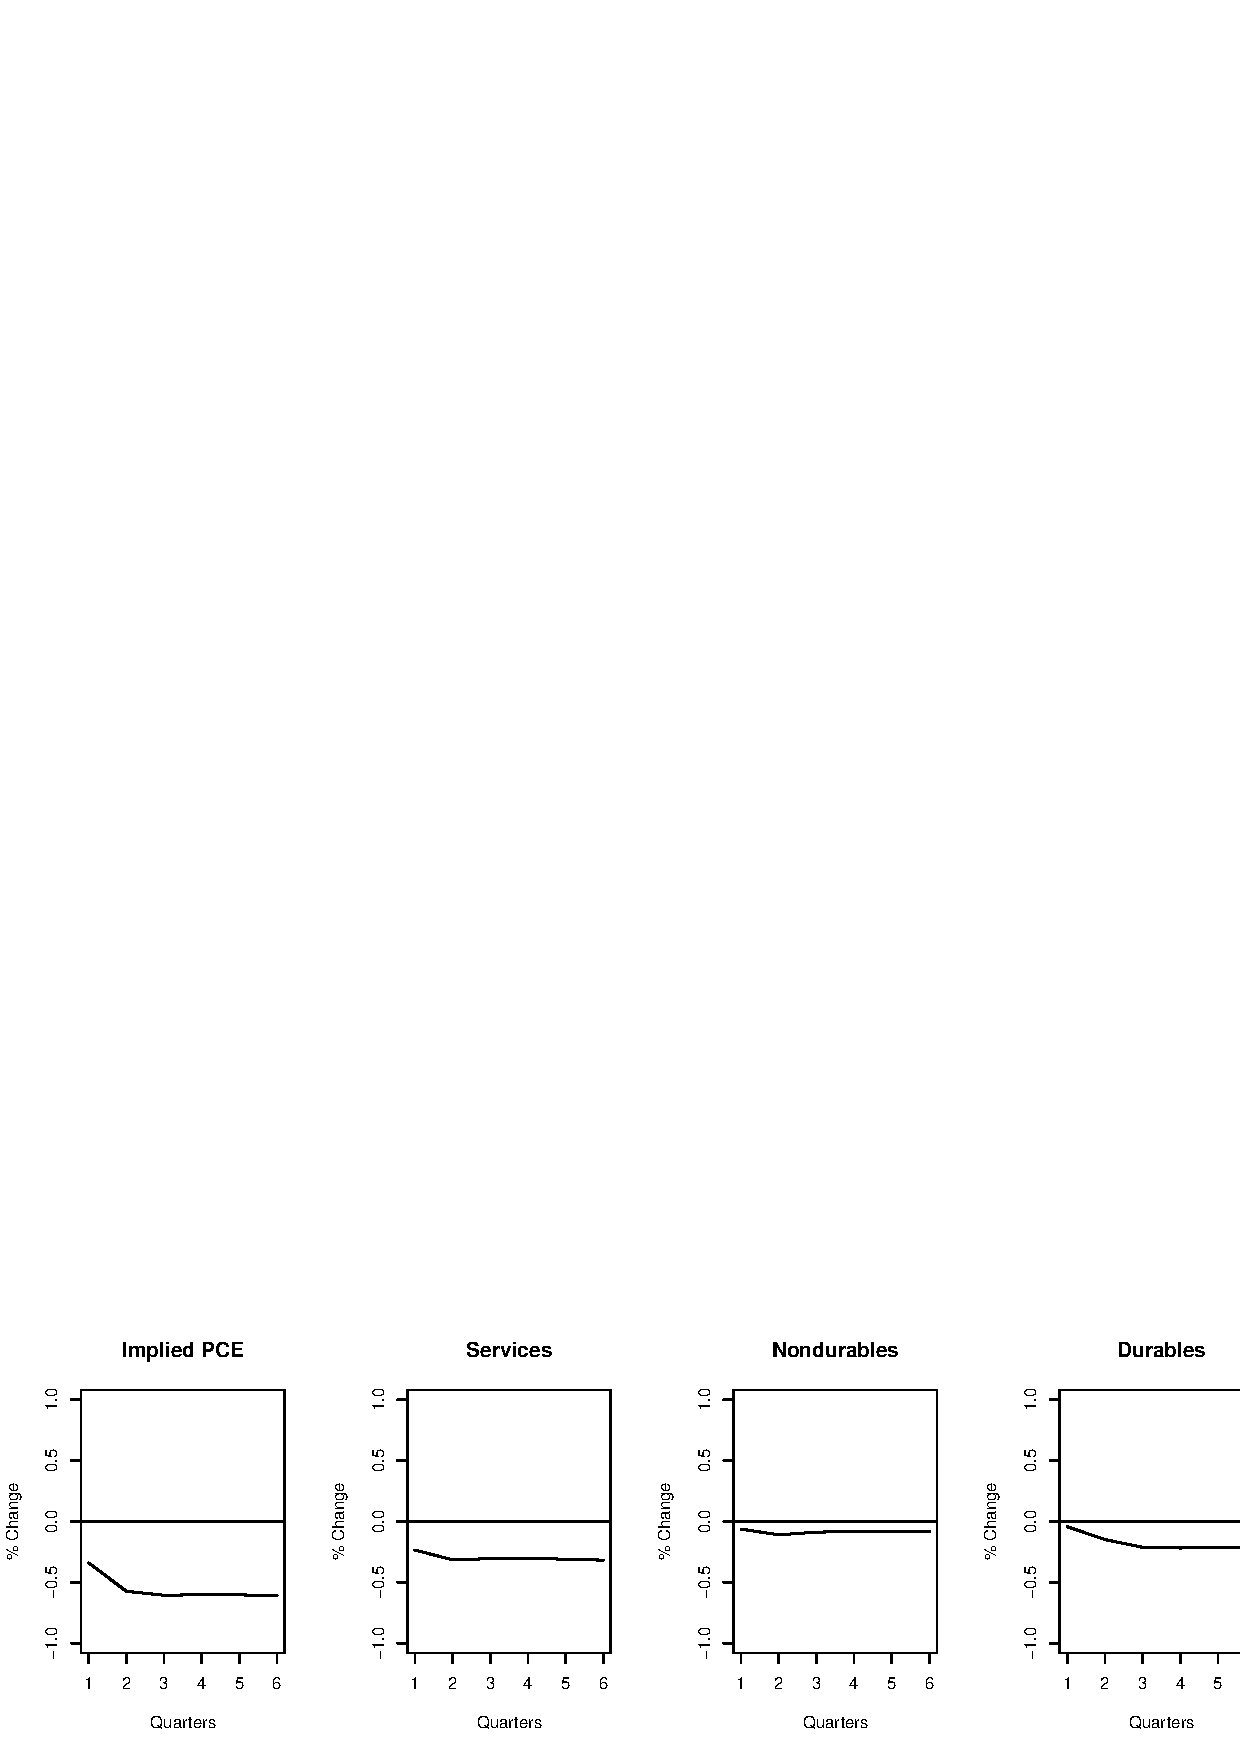
\includegraphics[width=0.55\textwidth,height=\textheight]{Contribution.png}
\caption{Contribution of each category in driving the response of
consumption.}
\end{figure}

\end{frame}

\begin{frame}{Interpretation of the Results}
\protect\hypertarget{interpretation-of-the-results}{}

\begin{itemize}
\item
  The average household income before taxes for 2017 was \$73,572, of
  which \$60,060 was used by households for consumption.
\item
  Based on our sample, consumers spend \$2,000 on gasoline and other
  energy goods.
\item
  Following a \$200 increase in gasoline expenditures across the course
  of the year, an average household reduces spending by \$389 over the
  same time period.
\item
  Services spending goes down by \$182, durables spending declines by
  \$123, and nondurables decreases by \$47.
\end{itemize}

\end{frame}

\begin{frame}{Other Categories of Consumption}
\protect\hypertarget{other-categories-of-consumption}{}

We also consider the following measures of consumption for our analysis:

\begin{itemize}
\tightlist
\item
  Durables

  \begin{itemize}
  \tightlist
  \item
    Furnishing Goods\\
  \item
    Motor Vehicles
  \item
    Recreational Goods
  \end{itemize}
\item
  Nondurables

  \begin{itemize}
  \tightlist
  \item
    Food and Beverages
  \item
    Clothing
  \end{itemize}
\item
  Services

  \begin{itemize}
  \tightlist
  \item
    Housing and Utilities
  \item
    Transportation
  \item
    Other (Communication, Education, etc)
  \end{itemize}
\end{itemize}

\end{frame}

\begin{frame}{Results: Other Categories of Consumption}
\protect\hypertarget{results-other-categories-of-consumption}{}

\begin{figure}
\centering
\includegraphics[width=0.8\textwidth,height=\textheight]{Disaggregated - 1.jpeg}
\caption{Response of consumption to a 10\% increase in gasoline
expenditures}
\end{figure}

\end{frame}

\begin{frame}{Results: Other Categories of Consumption}
\protect\hypertarget{results-other-categories-of-consumption-1}{}

\begin{figure}
\centering
\includegraphics[width=0.8\textwidth,height=\textheight]{Disaggregated - 2.jpeg}
\caption{Response of consumption to a 10\% increase in gasoline
expenditures}
\end{figure}

\end{frame}

\begin{frame}{Other Categories of Consumption}
\protect\hypertarget{other-categories-of-consumption-1}{}

\begin{itemize}
\item
  A \$200 annual increase in gasoline expenditures will force an average
  household to reduce spending on motor vehicles by \$82 over the course
  of a year.
\item
  Spending on furnishing and other durable household equipment, and
  clothing goes down by \$16 and \$10 respectively.
\item
  Spending on food stays at its original level.
\item
  Public transportation expenditures increase by \$9.
\item
  Expenditures on housing go down by \$57, whereas utility bills
  increase by \$11 over the course of a year.
\end{itemize}

\end{frame}

\begin{frame}{Crowding Out of Non-Gasoline Spending}
\protect\hypertarget{crowding-out-of-non-gasoline-spending}{}

\begin{itemize}
\item
  The bivariate VAR model results suggest that as gasoline expenditures
  increase, consumption falls.
\item
  This decline in consumption is refered to as the `discretionary income
  effect'.
\item
  Once consumers are done paying for gasoline and other gasoline goods,
  they have less money to spend on other goods and services.
\item
  These results are evidence that an increase in gasoline expenditures
  has the same effect as an increase in tax on consumers.
\end{itemize}

\end{frame}

\begin{frame}{Asymmetric Effects Over Business Cycle}
\protect\hypertarget{asymmetric-effects-over-business-cycle}{}

\begin{itemize}
\item
  We model the asymmetric response of consumption variables to gasoline
  expenditure shocks in recessions and expansions using local
  projections.
\item
  Local projections have the ability to accomodate nonlinear
  specification.
\item
  Estimating a linear model for each regime separately will make our
  estimates imprecise due to insufficient degrees of freedom for
  recessions.
\item
  On the other hand, a nonlinear model allows us to utilize the entire
  dataset for our analysis.
\end{itemize}

\end{frame}

\begin{frame}{Asymmetric Effects Over Business Cycle}
\protect\hypertarget{asymmetric-effects-over-business-cycle-1}{}

Assuming that consumption growth responds contemporaneously to an
increase in gasoline expenditures, the immediate response of consumption
growth, \(\Delta c_t\), to a gasoline expenditure shock can be estimated
with the following regressions.

\[\Delta c_{t}=\alpha+ \sum_{i=0}^{k}\phi_{i}I_{t-i}+\sum_{i=0}^{k}\theta_{i}\triangle y_{t-i}+\sum_{i=1}^{k}\beta_{i}\Delta c_{t-i}+\sum_{i=0}^{k}\gamma_{i}\triangle gas_{t-i}\]

\[+\sum_{i=0}^{k}\delta_{i}inter_{t-i}+\varepsilon_t\] Where,
\[inter_{t-i}=I_{t-i} \times \triangle gas_{t-i}\]

\end{frame}

\begin{frame}{Asymmetric Effects Over Business Cycle}
\protect\hypertarget{asymmetric-effects-over-business-cycle-2}{}

We follow AG (2012) and define a recession in the following manner,
\[I_{t}=\begin{cases}
1 & F(z_{t})\geq0.8\\
0 & F(z_{t})<0.8
\end{cases}\]

The transition function that indicates the state of the economy takes
the following functional form,
\[F(z_t)= \frac{exp(-\gamma (z_t-\bar{d}))}{1+exp(-\gamma (z_t-\bar{d}))}, \gamma>0.\]

Where \(z_t\) is equal to the seven quarter moving average growth rate
of output and the value of \(\gamma\) is calibrated to be equal to 3 so
that the economy spends 20\% of time in recession,
\[Pr(F(z_t)>0.8)=0.2\]

\end{frame}

\begin{frame}{Asymmetric Effects Over Business Cycle}
\protect\hypertarget{asymmetric-effects-over-business-cycle-3}{}

\begin{figure}
\centering
\includegraphics[width=0.9\textwidth,height=\textheight]{Recession.jpeg}
\caption{Estimated values of the AG (2012) transition function}
\end{figure}

\end{frame}

\begin{frame}{Asymmetric Effects Over Business Cycle}
\protect\hypertarget{asymmetric-effects-over-business-cycle-4}{}

Defining \(\Delta gas_0\) as the change in gasoline expenditures in
recessions and expansions, and \(inter_0\) as the change in gasoline
expenditures in recessions, the contemporaneous response of
\(\Delta c_t\), \(\Delta c_0\) is defined as
\[\Delta c_{0}=\hat{\gamma}_{0}\triangle gas_{0}+\hat{\delta}_{0}inter_{0}\]

\[\Delta c_{0}^{rec}=\hat{\gamma}_{0}\triangle gas_{0}+\hat{\delta}_{0}inter_{0}\]

\[\Delta c_{0}^{exp}=\hat{\gamma}_{0}\triangle gas_{0}\]

Since the shock under study is a 10\% increase in gasoline expenditures
\(\triangle gas_{0}=0.1\). For a 10\% shock in recessions,
\(inter_{0}=0.1\). For expansions, on the other hand, \(inter_{0}=0\)
since \(I_{t}=0\).

\end{frame}

\begin{frame}{Asymmetric Effects Over Business Cycle}
\protect\hypertarget{asymmetric-effects-over-business-cycle-5}{}

We then define the initial response vector for each regime,
\[d_{i}^{rec}=\begin{bmatrix}\Delta c_{0}^{rec} & \triangle gas_{0} & inter_{0}\end{bmatrix}\]

\[d_{i}^{exp}=\begin{bmatrix}\Delta c_{0}^{exp} & \triangle gas_{0} & 0\end{bmatrix}\]

The s-period impulse responses are then calculated by estimating a
reduced form regression,
\[\Delta c_{t}=\alpha+\sum_{i=1}^{k}\phi_{i}I_{t-i}+\sum_{i=1}^{k}\theta_{i}\triangle y_{t-i}+\sum_{i=1}^{k}\beta_{i}\Delta c_{t-i}+\sum_{i=1}^{k}\gamma_{i}\triangle gas_{t-i}\]
\[+\sum_{i=1}^{k}\delta_{i}inter_{t-i}+\varepsilon_{t}\]

\end{frame}

\begin{frame}{Asymmetric Effects Over Business Cycle}
\protect\hypertarget{asymmetric-effects-over-business-cycle-6}{}

The response for both regimes is calculated using the following,
\[\hat{IR}_{s}^{rec}=\Phi_{s}d_{i}^{rec}=\hat{\beta}_{s}\Delta c_{0}+\hat{\gamma}_{s}\triangle gas_{0}+\hat{\delta}_{s}inter_{0}\]

and
\[\hat{IR}_{s}^{exp}=\Phi_{s}d_{i}^{exp}=\hat{\beta}_{s}\Delta c_{0}+\hat{\gamma}_{s}\triangle gas_{0}\]

where
\[\Phi_{s}=\begin{bmatrix}\hat{\beta}_{s} & \hat{\gamma}_{s} & \hat{\delta}_{s}\end{bmatrix}\]

\end{frame}

\begin{frame}{Asymmetric Effects Over Business Cycle}
\protect\hypertarget{asymmetric-effects-over-business-cycle-7}{}

\begin{itemize}
\item
  Once we construct the impulse responses for both regimes, we can
  calculate the cumulative impulse response functions.
\item
  The rationale to use cumulative impulse responses is that it allows us
  to calculate the deviation of consumption from its' long-run level.
\end{itemize}

\[CIR_{s}^{rec}=\sum_{j=0}^{s}\widehat{IR}_{j}^{rec}\]

\[CIR_{s}^{exp}=\sum_{j=0}^{s}\widehat{IR}_{j}^{exp}\]

\end{frame}

\begin{frame}{Asymmetric Effects Over Business Cycle}
\protect\hypertarget{asymmetric-effects-over-business-cycle-8}{}

In order to calculate the asymmetric response of \(c_{t}\) to gasoline
expenditure shocks, we take the difference between the impulse responses
across recessions and expansions.

\[CIR_{s}^{rec}-CIR_{s}^{exp}=\sum_{j=0}^{s}\widehat{IR}_{j}^{rec}-\sum_{j=0}^{s}\widehat{IR}_{j}^{exp}\]

\[\triangle CIR_{s}=\sum_{j=0}^{s}\widehat{IR}_{j}^{rec}-\sum_{j=0}^{s}\widehat{IR}_{j}^{exp}\]

If \(\triangle CIR_{s}<0\), this means the response of consumption,
\(c_{t}\) is stronger in a recession as compared to an expansion.
\(\triangle CIR_{s}>0\) suggests the opposite.

\end{frame}

\begin{frame}{Results: Asymmetric Effects Over Business Cycle}
\protect\hypertarget{results-asymmetric-effects-over-business-cycle}{}

\begin{figure}
\centering
\includegraphics[width=0.6\textwidth,height=\textheight]{Asymmetry - Aggregated.png}
\caption{Response of consumption to a 10\% increase in gasoline
expenditures. Solid line is the response in a recession, whereas the
corresponding dashed line is the response in an expansion.}
\end{figure}

\end{frame}

\begin{frame}{Results: Asymmetric Effects Over Business Cycle}
\protect\hypertarget{results-asymmetric-effects-over-business-cycle-1}{}

\begin{itemize}
\item
  Non-gasoline consumption decreases by around 2\% more in recessions as
  opposed to in expansions.
\item
  Durables PCE decreases by almost 5.20\% more following the shock in
  recessions.
\item
  The difference in response among nondurables and services is -1.45\%
  and -1.43\% respectively.
\item
  The highly elastic nature of durable goods explains the big drop.
\end{itemize}

\end{frame}

\begin{frame}{Results: Asymmetric Effects Over Business Cycle}
\protect\hypertarget{results-asymmetric-effects-over-business-cycle-2}{}

\begin{figure}
\centering
\includegraphics[width=0.6\textwidth,height=\textheight]{Difference - Aggregated.png}
\caption{Solid line represents the difference in response, whereas the
corresponding dashed line is the 95\% confidence interval.}
\end{figure}

\end{frame}

\begin{frame}{Results: Asymmetric Effects Over Business Cycle}
\protect\hypertarget{results-asymmetric-effects-over-business-cycle-3}{}

\begin{figure}
\centering
\includegraphics[width=0.8\textwidth,height=\textheight]{Asymmetry - 1.jpeg}
\caption{The top row indicates the response of consumption to a 10\%
increase in gasoline expenditures, whereas the lower row represents the
difference in response across regimes with the corresponding dashed
lines are the 95\% confidence interval.}
\end{figure}

\end{frame}

\begin{frame}{Results: Asymmetric Effects Over Business Cycle}
\protect\hypertarget{results-asymmetric-effects-over-business-cycle-4}{}

\begin{figure}
\centering
\includegraphics[width=0.8\textwidth,height=\textheight]{Asymmetry - 2.jpeg}
\caption{The top row indicates the response of consumption to a 10\%
increase in gasoline expenditures, whereas the lower row represents the
difference in response across regimes with the corresponding dashed
lines are the 95\% confidence interval.}
\end{figure}

\end{frame}

\begin{frame}{Results: Asymmetric Effects Over Business Cycle}
\protect\hypertarget{results-asymmetric-effects-over-business-cycle-5}{}

\begin{figure}
\centering
\includegraphics[width=0.8\textwidth,height=\textheight]{Asymmetry - 3.jpeg}
\caption{The top row indicates the response of consumption to a 10\%
increase in gasoline expenditures, whereas the lower row represents the
difference in response across regimes with the corresponding dashed
lines are the 95\% confidence interval.}
\end{figure}

\end{frame}

\begin{frame}{Interpretation of the Results}
\protect\hypertarget{interpretation-of-the-results-1}{}

\begin{itemize}
\item
  In dollar terms, a \$200 increase in gasoline expenditures for any
  year reduces total non-gasoline spending for an average household by
  \$1,545 in recessions and \$383 in expansions.
\item
  Durables lose out by \$530 in recessions as opposed to \$137 in
  expansions.
\item
  Spending on nondurables decreases by \$249 in recessions and \$55 in
  expansions.
\item
  On the other hand, services spending goes down by \$689 in recessions
  as opposed to \$156 in expansions.
\end{itemize}

\end{frame}

\begin{frame}{Source of Asymmetry}
\protect\hypertarget{source-of-asymmetry}{}

\begin{itemize}
\item
  Precautionary Savings Effect: Edelstein and Kilian (2009)
\item
  We reestimate the nonlinear model using personal savings as the
  dependent variable,
  \[Personal\;Savings=Disposable\;Income-Personal\;Outlays. \]
\item
  The estimates from our model suggest that a 10\% increase in gasoline
  expenditures over the course of a year increases savings by 3.57\% in
  recessions as opposed to 0.92\% in expansions.
\end{itemize}

\end{frame}

\begin{frame}{Source of Asymmetry}
\protect\hypertarget{source-of-asymmetry-1}{}

\begin{itemize}
\item
  The difference in response of savings indicates that the precautionary
  savings channel is amplified in recessions.
\item
  A \$200 increase in gasoline expenditures increases private savings by
  \$398 in recessions and \$60 in expansions.
\item
  As gasoline expenditures increase in recessions, consumers become
  skeptical about the future path of the economy.
\item
  Consumers increase their savings by more because they perceive a
  higher likelihood of unemployment during recessions.
\end{itemize}

\end{frame}

\begin{frame}{Why Should We Care? (Change)}
\protect\hypertarget{why-should-we-care-change}{}

\begin{itemize}
\item
  A finding of economically meaningful asymmetry of requires a change to
  empirical and theoretical macroeconomic models that include energy
  prices.
\item
  This suggests that the Federal Reserve's consumption forecasting
  models need to account for this asymmetric behaviour.
\item
  Forecasts with the linear model might underestimate the effects of
  gasoline expenditure shocks. (Add details about models being
  forecasted.)
\end{itemize}

\end{frame}

\begin{frame}{Forecasting Implications}
\protect\hypertarget{forecasting-implications}{}

\begin{figure}
\centering
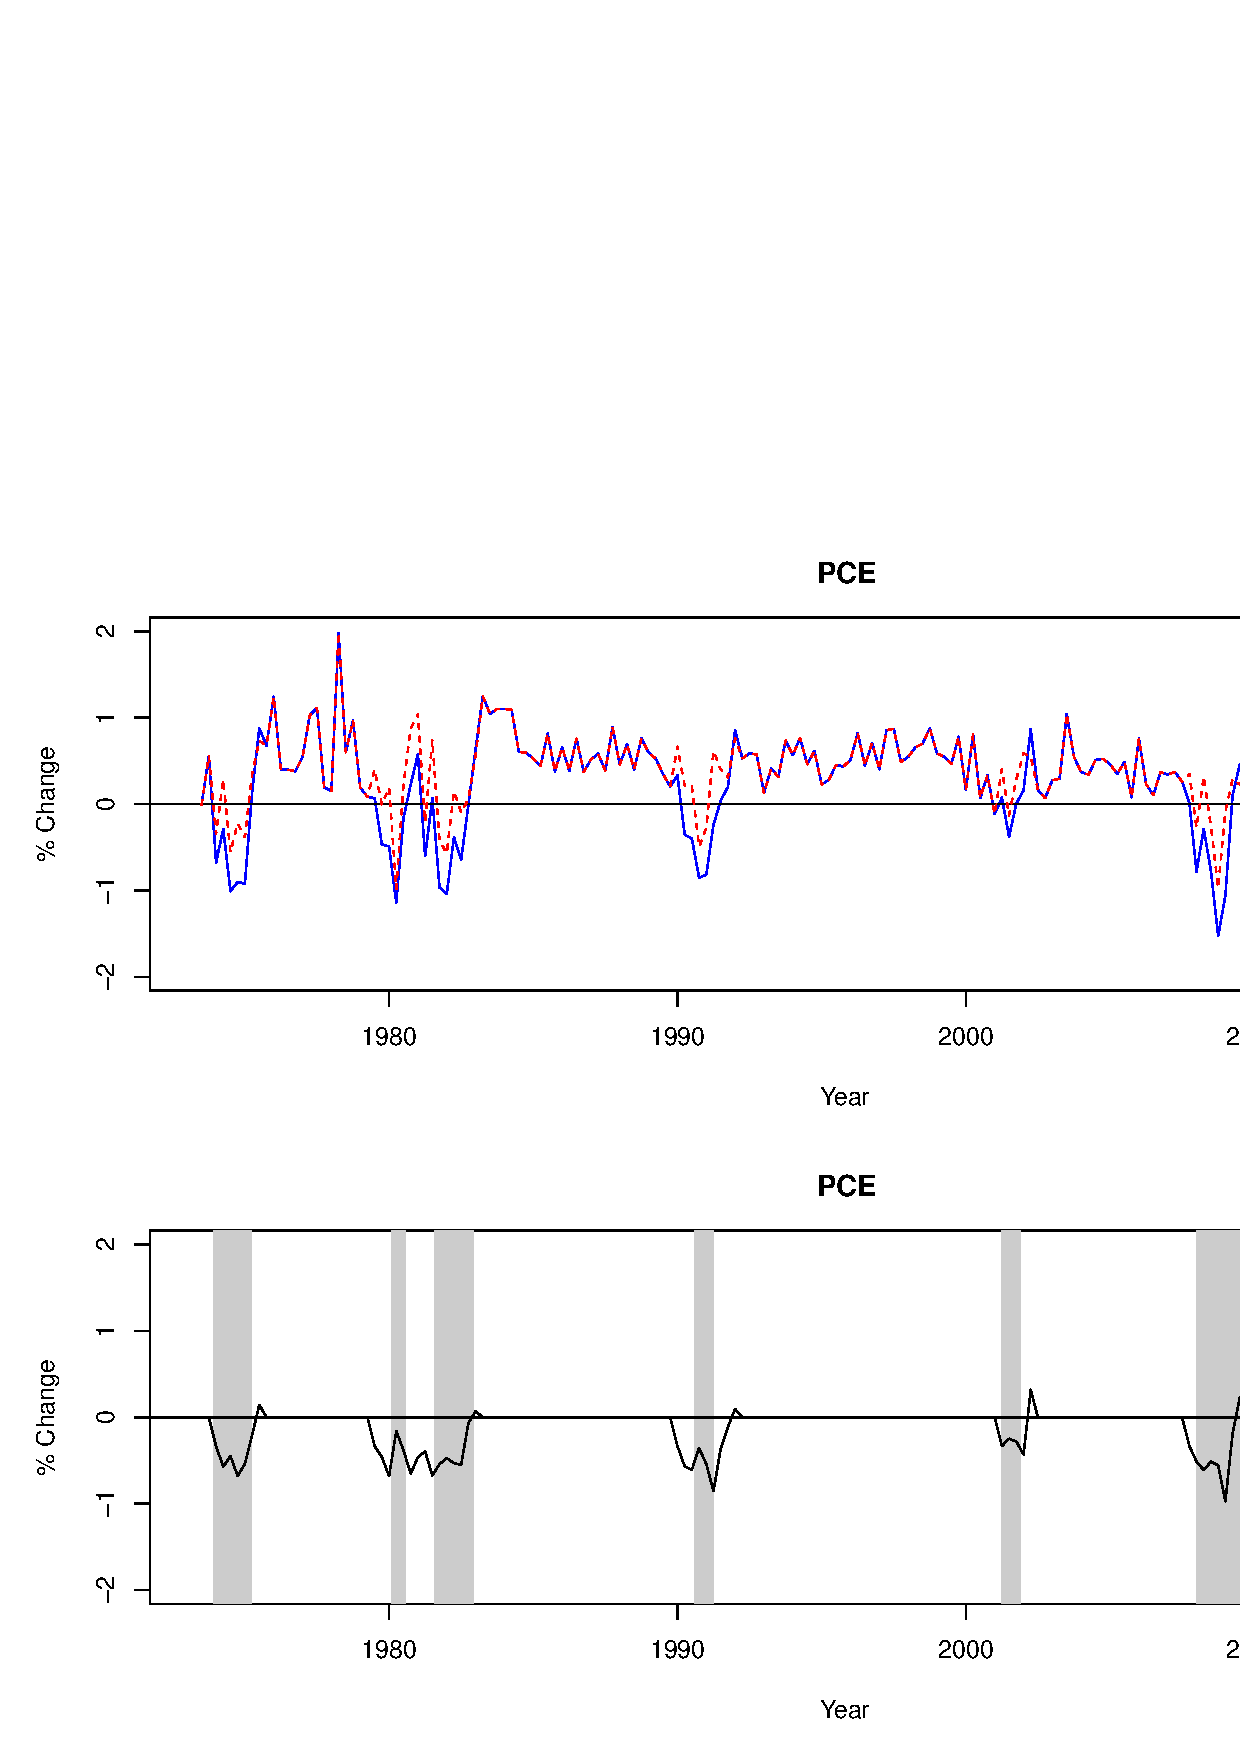
\includegraphics[width=0.85\textwidth,height=\textheight]{Forecasts - PCE.jpeg}
\caption{Consumption forecasts following a 10\% increase in gasoline
expenditures.}
\end{figure}

\end{frame}

\begin{frame}{Forecasting Implications}
\protect\hypertarget{forecasting-implications-1}{}

\begin{figure}
\centering
\includegraphics{Nondurables Services.jpeg}
\caption{Consumption forecasts following a 10\% increase in gasoline
expenditures.}
\end{figure}

\end{frame}

\begin{frame}{Alternative Recession Dates}
\protect\hypertarget{alternative-recession-dates}{}

\begin{itemize}
\item
  Different measures of recessions have been proposed in the literature,
  i.e.~unemployment rate, capacity utilization, and output gap.
\item
  We reestimate our model using an alternative recession date proposed
  by Hamilton.
\item
  Hamilton like AG (2012), also estimates recession dates,
  \[P(Recession|GDP)=\frac{P(Recession\bigcap GDP)}{P(GDP)}\]
\end{itemize}

\end{frame}

\begin{frame}{Alternative Recession Dates (Change)}
\protect\hypertarget{alternative-recession-dates-change}{}

\begin{figure}
\centering
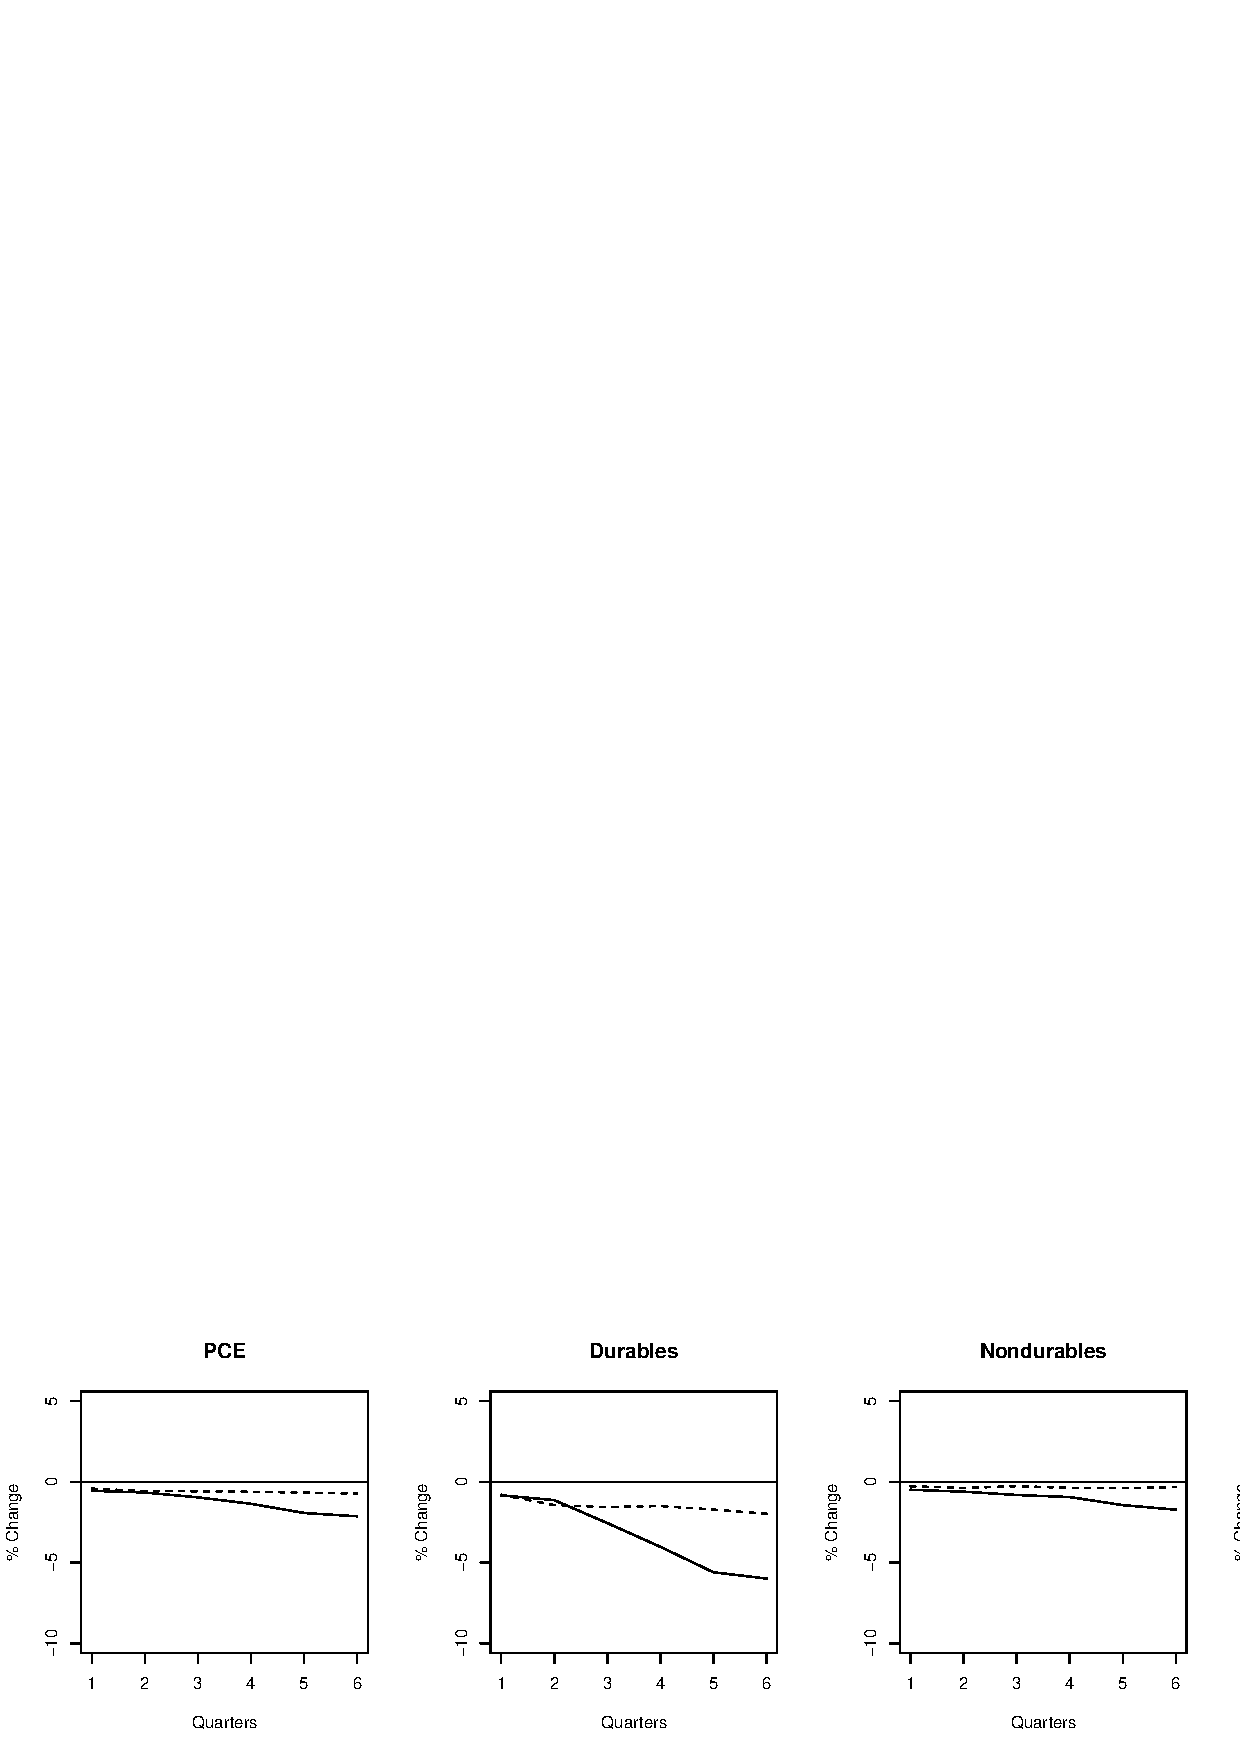
\includegraphics[width=0.7\textwidth,height=\textheight]{Hamilton.png}
\caption{Responses and Difference in Response.}
\end{figure}

\end{frame}

\begin{frame}{Alternative Measure of Shock}
\protect\hypertarget{alternative-measure-of-shock}{}

\begin{itemize}
\tightlist
\item
  We also redo the analysis using real price of gasoline.
\end{itemize}

\[\Delta c_{t}=\alpha+ \sum_{i=0}^{k}\phi_{i}I_{t-i}+\sum_{i=0}^{k}\theta_{i}\triangle y_{t-i}+\sum_{i=1}^{k}\beta_{i}\Delta c_{t-i}+\sum_{i=0}^{k}\gamma_{i}\triangle rpg_{t-i}\]

\[+\sum_{i=0}^{k}\delta_{i}inter_{t-i}+\varepsilon_t\] Where,
\[inter_{t-i}=I_{t-i} \times \triangle rpg_{t-i}\]

\end{frame}

\begin{frame}{Alternative Measure of Shock (Change)}
\protect\hypertarget{alternative-measure-of-shock-change}{}

\begin{figure}
\centering
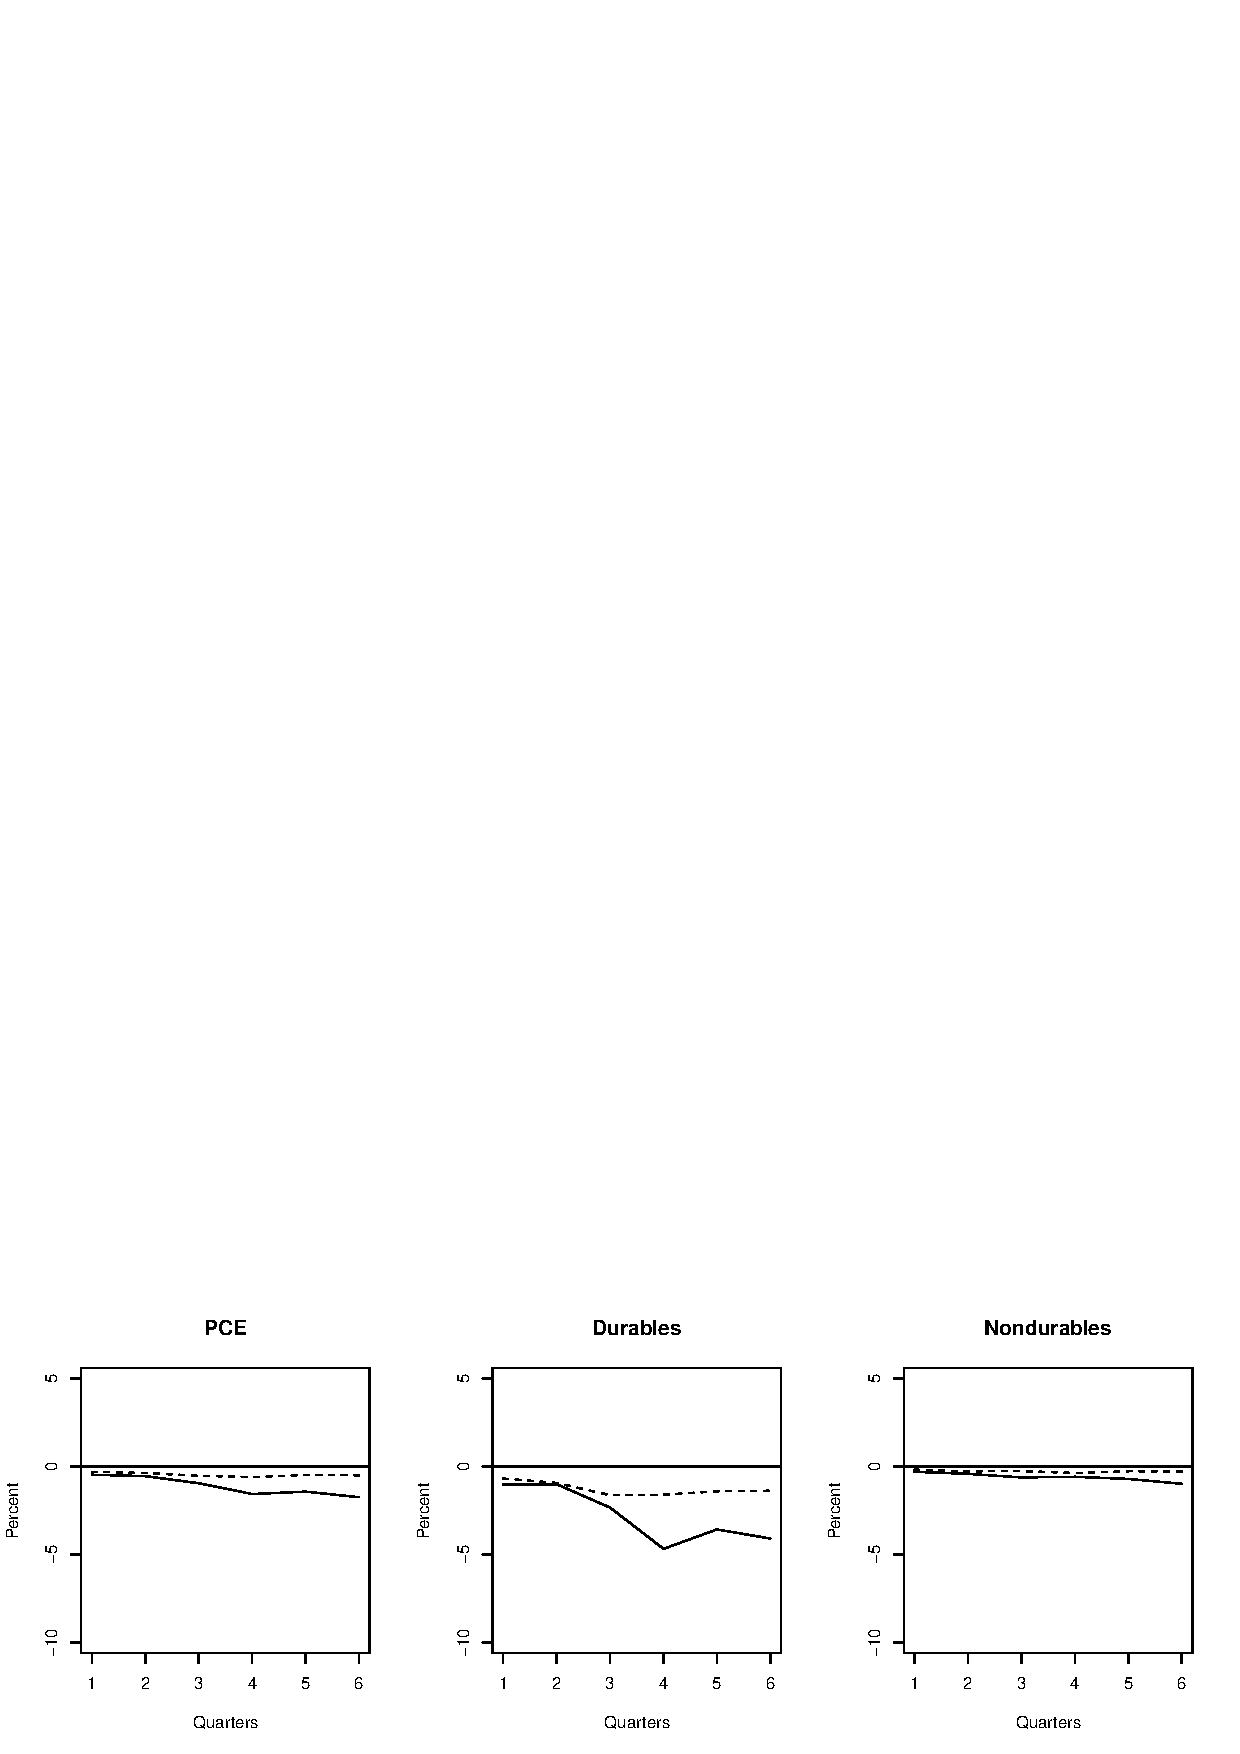
\includegraphics{RPG.jpg}
\caption{Response of consumption to a 10\% increase in real price of
gasoline.}
\end{figure}

\end{frame}

\begin{frame}{Positive versus Negative Shocks}
\protect\hypertarget{positive-versus-negative-shocks}{}

\begin{itemize}
\item
  We also consider the response of consumption to negative gasoline
  expenditure shocks.
\item
  Oil price decreases cause a transfer of wealth from oil-exporting to
  oil-importing countries.
\item
  A decrease in gasoline expenditures frees up a portion of income,
  consequently, increasing spending on non-gasoline goods and services.
\end{itemize}

\end{frame}

\begin{frame}{Positive versus Negative Shocks}
\protect\hypertarget{positive-versus-negative-shocks-1}{}

\begin{figure}
\centering
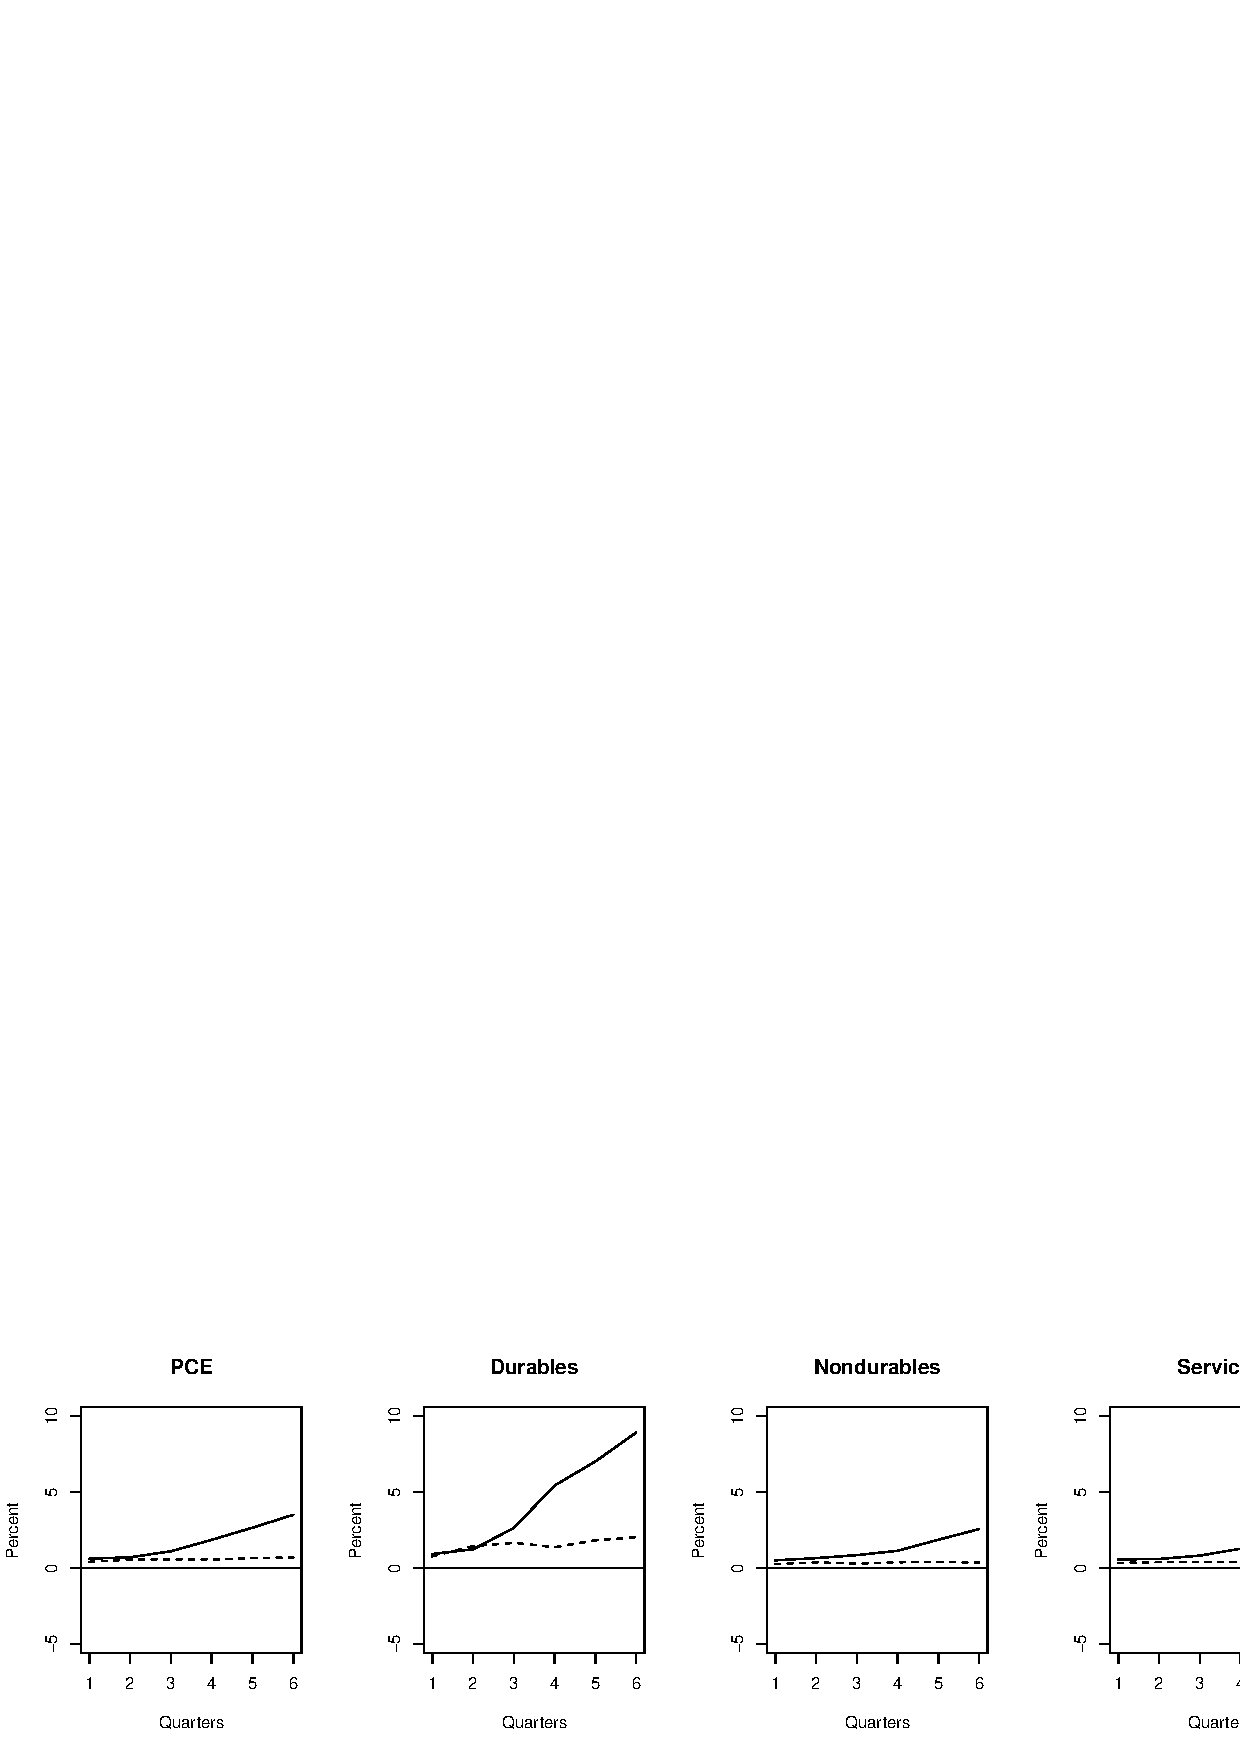
\includegraphics{Decreases.jpg}
\caption{Response of consumption to a 10\% decrease in gasoline
expenditures.}
\end{figure}

\end{frame}

\begin{frame}{Conclusion}
\protect\hypertarget{conclusion}{}

\begin{itemize}
\item
  An increase in gasoline expenditures has the same effect as a tax on
  U.S. consumers, because it transfers a portion of theirincome to
  foreign oil producers and depresses non-gasoline consumption.
\item
  We find evidence that the effect of a gasoline expenditure shock
  depends on the state of the business cycle.
\item
  The response to a gasoline expenditure shock is much stronger in a
  recession than in an expansion.
\item
  We present a forecasting model that accounts for the asymmetric
  behaviour of consumption to a gasoline expenditure shock across
  recessions and expansions.
\end{itemize}

\end{frame}

\begin{frame}{Conclusion}
\protect\hypertarget{conclusion-1}{}

\begin{itemize}
\item
  The difference in response over the business cycle is due to the
  differences in household savings behaviour in recessions versus
  expansions.
\item
  Our central estimates are robust to alternative measure of recession
  and shock as well.
\item
  The extra income generated following a decrease in gasoline
  expenditures is more effective in boosting consumption during
  recessions.
\end{itemize}

\end{frame}

\begin{frame}{Thank You.}
\protect\hypertarget{thank-you.}{}

\begin{center}
Questions?
\end{center}

\end{frame}

\end{document}
